\chapter{Experiments and Evaluation}
\label{sec:experiments}

The general idea behind the upcoming experiments is the following simple scheme: Problem simulation by publishing on the respective topic, followed by a triggered monitoring
procedure that should detect the problem, interrupt normal operation and initiate an appropriate resolution. Either it succeeds and \code{NORMAL_OPERATION} continues, or it cannot be
resolved and execution ends in \code{CATASTROPHE}.\newline
Hawes et al. introduce two useful metrics to evaluate the performance of a long-term autonomous system: The \textit{total system lifetime} and the \textit{autonomy percentage}. \cite{Hawes:2017} The
first measures the time the robot is in autonomous operation and is reset when an unsolvable problem or an unintended intervention of the human operator is required. However,
it is not reasonable to evaluate this time in the present scenario, since it certainly depends on the frequency with which the failures considered in this work are simulated. The second metric
(autonomy percentage), on the other hand, is very useful for this thesis as well. \textquote{\textit{The motivation of the autonomy percentage is that it is of little value to achieve a long
total system lifetime if the system does nothing}}. \cite{Hawes:2017}
Steinberg et al. \cite{Steinberg:2016} introduce the metric of time between undesired human interventions. By undesired interventions, they mean situations in which the robot should
in principle be able to recover itself, as opposed to situations in which human intervention is expected. Applied to this work, this could refer to LTA failures for which specific
solutions or workarounds have been proposed (cf. sec. \ref{sec:solutions_for_lta_challenges}) but have not been successful. In the following sections, this would manifest in
simulated contingency situations ending in a catastrophe. Furthermore, they propose a metric for information sharing, i.e., the percentage of time the robot communicates meaningful
information to the operator. This is definitely fulfilled by the presented approaches, in particular by the bidirectional communication channel between the robot and the human
operator (cf. sec. \ref{sec:fallback_solution}) and the \code{data_accumulator} (cf. sec. \ref{sec:black_box}). In any situation identified as problematic, meaningful information
is provided about the circumstances and the nature of the problem as such. Based on the developed architecture, this boils down to a question of reliability, which is evaluated in
section \ref{sec:eval_mon_framework}. If the problem at hand is properly identified, meaningful information will be provided with certainty.\newline

\noindent
Initially, the basic functionality of the entire integrated system is demonstrated in section \ref{sec:demonstration_of_functionality}. Subsequently, in section
\ref{sec:classification_of_lta_problems}, the identified problem categories are classified according to their severity. Eventually, section \ref{sec:eval_mon_framework} deals with
assessing the reliability of the presented monitoring solutions. All experiments were performed on an \textsf{Intel\textsuperscript{\textregistered} Core\texttrademark $\thinspace$
i7-6700K} system equipped with \textsf{48 GB RAM} running \textsf{Ubuntu 20.04}.

\section{Functionality of the Integrated System}
\label{sec:demonstration_of_functionality}

In order for the evaluation to be reasonably meaningful, the experiments must be of a certain length. At the same time, they must be feasible within the restrictive time constraints
of this thesis. As a compromise, the time per run was set to $5$ hours. Experimentally, it turned out that this runtime is sufficient to achieve a certain validity, since several
mission and charge cycles occur and there is enough room for error simulation (cf. sec. \ref{sec:eval_mon_framework}). Obviously, the number of missions that take place during this
period depends on the plan that defines such a mission. The complete plan underlying the experiments, executed in a loop, can be found in the appendix (cf. sec.
\ref{sec:complete_plan_sec}). The rationale behind the plan is that it incorporates all aspects relevant to the baseline scenario of long-term autonomy presented in section
\ref{sec:prototype_scenario}. It essentially satisfies the constraints for a long-term autonomous operation that are defined in section \ref{sec:lta_plant_observation}, e.g., it is
long enough to require several charge stops, and contains all the introduced actions (cf. sec. \ref{sec:plan_generation}). In addition, it provides a variety of situations
through different places that are approached.\newline

\noindent
The very first step is to show that without simulating any of the identified LTA problems, the mission runs flawlessly for the previously motivated $5$ hours. This serves as
a verification of the plan, i.e., it shows that the charging stops are sufficient if everything works as expected. Furthermore, it is a demonstration of the fundamental
functionality of the entire integrated system in the absence of unexpected problematic events. For evaluation purposes, let a failed mission be defined as a mission that exceeds a
user-configurable timeout $t = 900s$ without publishing a message to \code{/arox/ongoing_operation}, although the previous message contained a value of \code{total_tasks} that is
greater than one, indicating that the current plan is not completed and thus that the robot has been stuck in that task for a time greater than $t$. Obviously, a \code{severe_failure}
in the low-level state machine leading to a transition to \code{CATASTROPHE} followed by a system shutdown is also considered a failed mission (cf. sec. \ref{sec:execution_monitoring_smach_architecture}). This would be the result of a completely
discharged battery. To endow this test of basic functionality with some significance, it was performed three times. Most importantly, all runs were completed without failure. Thus,
unsurprisingly, the average runtime is $5.09$ hours. In this time, the robot has completed an average of $3.67$ missions and $106.67$ tasks. It required an average of $9.67$
charge cycles and the average total distance traveled is $1102.68 m$. Moreover, it is interesting to look at the mode distribution, i.e., how long the robot was in which mode
during the LTA episodes, which is shown in fig. \ref{fig:mode_times_basic}.

\vfill
\pagebreak

\begin{figure}[H]
    \centering
    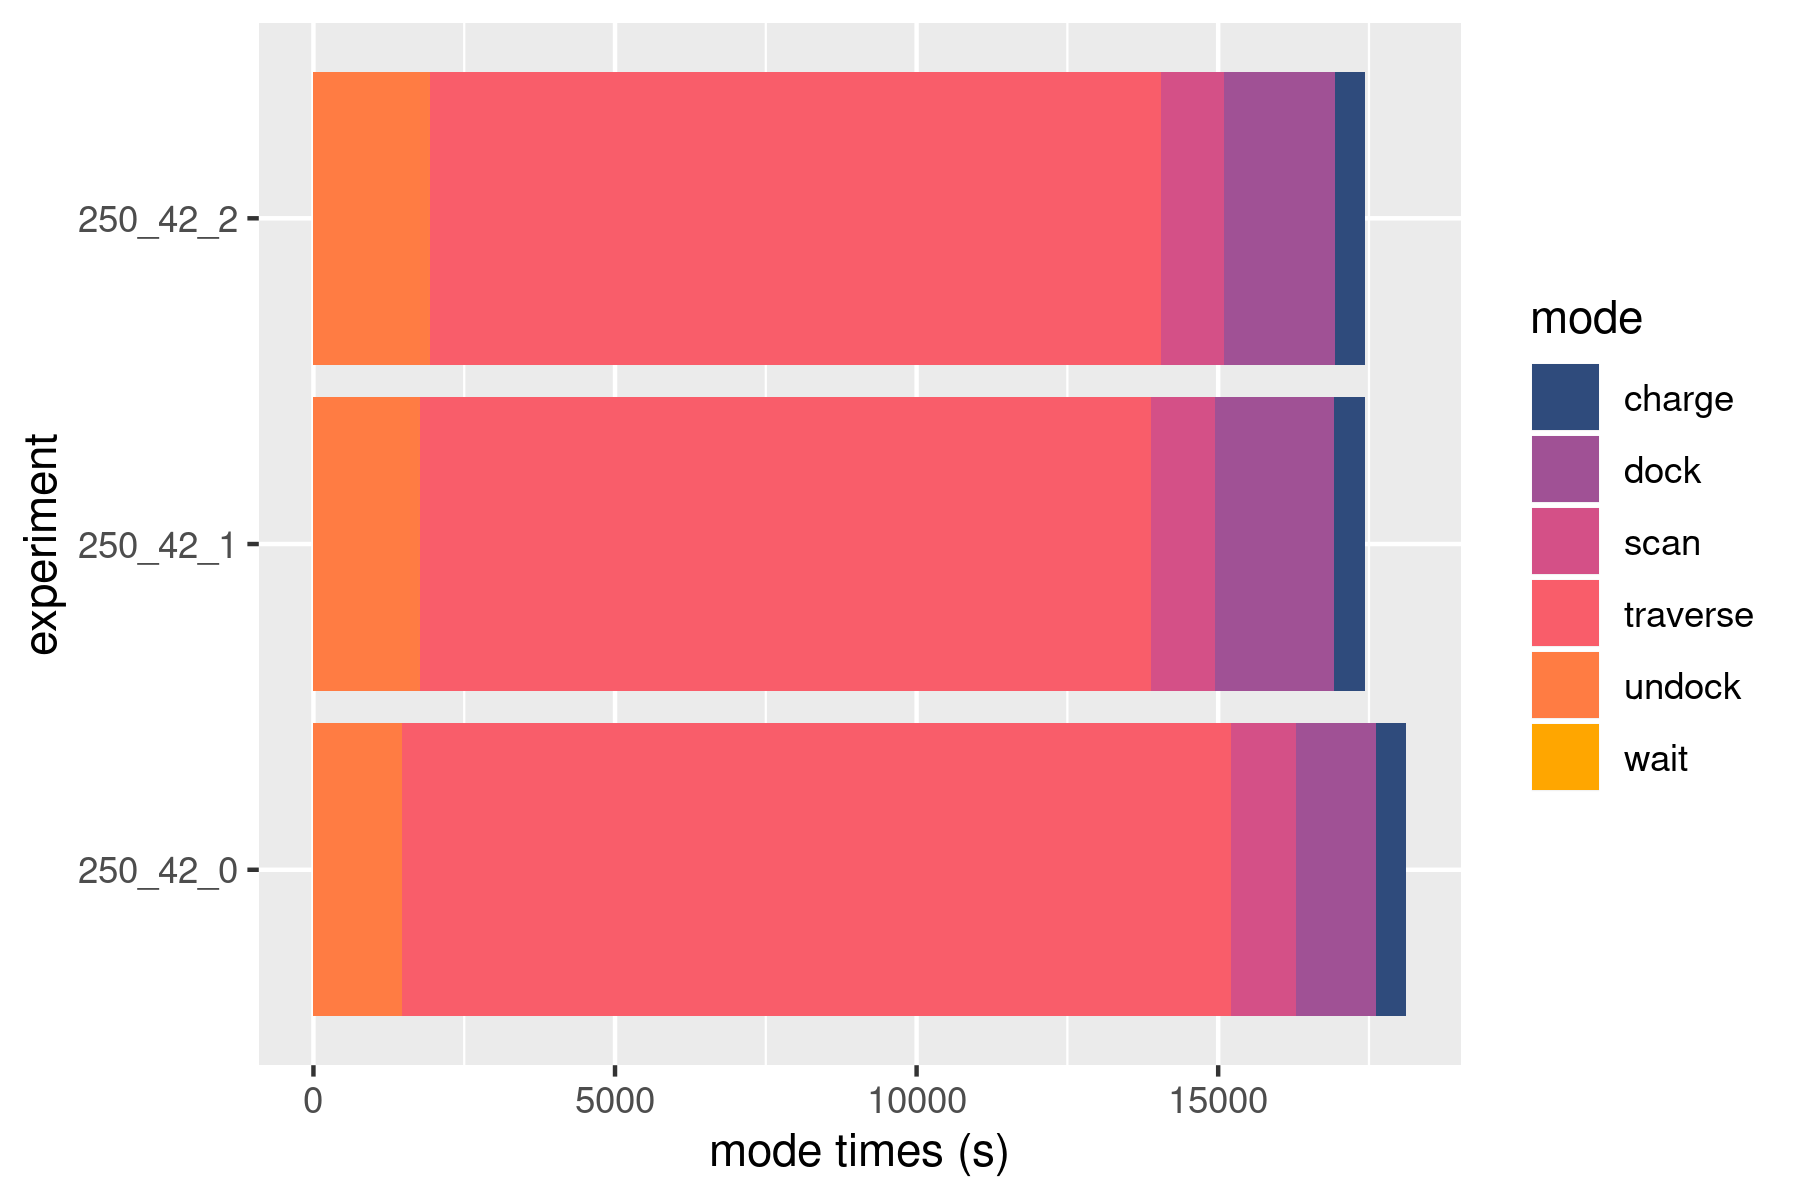
\includegraphics[width=0.525\textwidth]{img/mode_times_basic.png}
    \caption{\textsc{Mode Distribution}}
    \label{fig:mode_times_basic}
\end{figure}
\noindent
Note that the robot spends hardly any time waiting and most of its time driving and scanning. Besides that, (un)docking and recharging naturally takes some time as well.
The relatively slight discrepancy in the results (completed tasks, missions, charge cycles, etc.) between runs arises from the fact that, for instance, the docking procedure does not always detect the container
at the same speed. In general, the simulation has certain non-deterministic aspects in the sense that the combination of all the ROS nodes, their communication, possible effects in
the simulation and execution times mean that two runs of such an experiment in simulation will certainly not be exact reproductions of the same states. Although the three runs do not
guarantee a fundamentally error-free use of the system, they demonstrate that the basic expected stable functionality is given.
The detailed results can be found in the appendix (cf. fig. \ref{fig:detailed_functionality_res}).

\section{Classification of the Selected LTA Problems}
\label{sec:classification_of_lta_problems}

A crucial question is whether the simulations of the problem cases presented in section \ref{sec:sim_and_mon_of_lta_challenges} are indeed representative of the problems in reality.
Oftentimes, the simulated cases exactly coincide with the actual cases in reality, e.g., in the case of extreme weather events, as it is simply a matter of data processing.
Otherwise, it ultimately boils down to the question of how compelling the argumentation is in the individual case.
The classification of the selected LTA challenges is based on their evaluation in the simulation together with a comparative contextualization of the practical case. The aim is to
classify the identified problem categories in the simulation according to their severity, i.e., which LTA challenge can lead to which worst-case outcome. By definition, all identified
problems can lead to contingencies, as outlined in the corresponding sections (cf. section \ref{sec:sim_and_mon_of_lta_challenges}). Additionally, all of them can lead to
catastrophes, at least as a fallback option in case of resolution failures. However, this implies monitoring to detect the issues. As a brief recap, contingencies are situations in
which the robot's ability to act is essentially preserved, so that it can attempt to solve the problem itself. Catastrophes, on the other hand, definitely require human intervention.
Hence, when the proposed monitoring framework is active, each problem category can potentially lead to the worst case outcome of \code{CATASTROPHE}. More interesting in terms of
classification is the present state of the AROX system, i.e., no monitoring for the identified issues. In this case, \code{CATASTROPHE} refers to one of the two aforementioned
conditions - battery failure or timeout - and is thus equivalent to mission abort. The first category is LTA problems that, when they occur, prevent the successful continuation of the
mission in the simulation. Despite the fact that it is evident for some of the identified problems for LTA operations, e.g., power management failures, that they are capable of
interrupting the mission, it is systematically investigated how the system in simulation responds to these failure cases without the developed monitoring procedures. This is critical to verify the
correct and expected behavior of the simulated fault cases.\newline

\noindent
Power management failures are the first case to be considered. When simulating a power management failure, e.g., by
publishing on \code{/sim_power_management_catastrophe}, the battery discharge rate is increased without the robot noticing, so it simply runs out of battery and normal operation
ends with a \code{severe_failure}, leading to a transition to \code{CATASTROPHE} and then a system shutdown. Thus, the simulation of power management failure works as expected. That
the general error class of charging failures can lead to a failed mission can be demonstrated by simulating a docking error that results in not being able to recharge and also
ends in \code{CATASTROPHE}. Hence, without active monitoring, \code{/sim_docking_failure_raised_ramp} is used to verify this. As expected, this also ends with a completely
discharged battery and thus a failure of the mission. Evidently, both cases lead to a failed deployment in practice with the real robot as well, which would go unnoticed without
monitoring.\newline

\noindent
The first example that cannot interfere with the operation in the simulation is drastic weather changes. Since these phenomena are not explicitly simulated in
\textit{Gazebo}, but are only indicated by corresponding messages on the weather monitoring channels, without active monitoring for these messages, the robot simply does not recognize
this. The same is true in practice: The robot would continue its mission without detecting a change in circumstances. Therefore, the mission would continue as long as possible, that
is, as long as the robot is not damaged. This is of course highly risky and can result in the robot being damaged or the sensor data being worthless. Consequently, it is apparent that
the monitoring of these phenomena is necessary. However, drastic weather changes per se will never lead to a catastrophe. Naturally, if the robot gets damaged, catastrophic
situations could occur, indirectly caused by drastic weather changes. Analogously, without the active monitoring, errors in sensor perception and data management would simply be
disregarded and go unnoticed. The robot's operation is not affected, but the results are of course worthless or not even saved, both in practice and in simulation. The
connection-related failures can be considered separately. WiFi outages do not affect the mission in the simulation, and in practice it depends on the exact use of the connection in
the considered scenario. If the RTK correction signal is sent via WiFi, localization may be compromised.  Additionally, if the scans are transferred via WiFi, the results may be lost
and the entire mission may become a futility. The same applies to an internet connection, where several parts of the system can be affected. Finally, GNSS-related failures can
directly lead to navigation failure even in simulation. For instance, \code{/sim_teleport}, which manipulates the latitude or longitude estimates, can drastically
falsify the robot's localization and cause arbitrarily severe failures. The robot could travel in dangerous or unsuitable places, or it could simply find itself in a situation that it
cannot leave and, in the best case, completely discharges its battery, leading to \code{CATASTROPHE} or to the fact that it can no longer perform any tasks, so that the mission fails
due to the timeout criterion introduced above. Moreover, plan distribution errors or navigation failures such as obstacles surrounding the robot, e.g., the \textquote{robot prison}
case in section \ref{sec:sim_and_mon_navigation_failures}, are simply not detected, but the mission can fail due to the timeout criterion or a completely discharged battery
(\code{CATASTROPHE}), whichever comes first. Failure is guaranteed for plan distribution errors and possible for navigation errors. This again holds for simulation as well as for
practice. That localization errors can have dramatic consequences up to \code{CATASTROPHE}
cases has already been shown by the example of GNSS connection issues.\newline

\noindent
The findings of the classification are summarized in fig. \ref{fig:lta_classification}. Crucially, any problem
category that has a \textquote{\cmark} or \textquote{(\cmark)} in the catastrophe column has the potential to abort the mission without monitoring solutions. Assuming persistent
failures, \textquote{\cmark} means that mission abort is a certainty, while \textquote{(\cmark)} stands for the possibility. Another perspective is that \textquote{\cmark} refers to
catastrophes caused directly by the problem, the problem itself causes the failure, not some effect on another aspect of the system, whereas \textquote{(\cmark)} stands for indirect
causation. Furthermore, the remaining problems of drastic weather changes, sensor failures and data management issues do not interrupt the mission, but they do invalidate the results
and thus have the potential to render the mission worthless both in practice and in simulation. There is only one exception: Drastic weather changes in the simulation. As already
anticipated, the actual occurrence of such events is not simulated, only the information of their presence. However, since the practical relevance is obvious, there is no need for
further simulation of e.g. impaired scans due to bad weather conditions. In summary, all of the identified issues have the potential to render LTA deployments worthless in real-world
scenarios, clearly highlighting the importance of addressing all of these problems if one aims to operate robots long-term autonomously in an outdoor context.
\begin{figure}[H]
    \centering
    \resizebox{\textwidth}{!}{
    \begin{tabular}{| c | c | c | c | c |}
        \hline
        \textbf{problem} & \specialcell{\textbf{contingency \& catastrophe} \\ \small{\textit{(with monitoring)}} \\ sim / prac} & \specialcell{\textbf{catastrophe} \\ \small{\textit{(without monitoring)}} \\ sim \quad\quad\quad\quad prac} & \specialcell{\textbf{potential to render mission worthless} \\ sim \quad\quad\quad\quad prac} \\ \hline
        power\_management & \cmark & \cmark \quad\quad\quad\quad\quad \cmark & \cmark \quad\quad\quad\quad\quad \cmark \\ \hline
        charging\_failure & \cmark & \cmark \quad\quad\quad\quad\quad \cmark & \cmark \quad\quad\quad\quad\quad \cmark \\ \hline
        drastic\_weather\_change & \cmark & \thinspace\thinspace \xmark \quad\quad\quad\quad\quad (\cmark) & \xmark \quad\quad\quad\quad\quad \cmark \\ \hline
        sensor\_failure & \cmark & \xmark \thinspace\thinspace\quad\quad\quad\quad\quad \xmark & \cmark \quad\quad\quad\quad\quad \cmark \\ \hline
        data\_management & \cmark & \xmark \thinspace\thinspace\quad\quad\quad\quad\quad \xmark & \cmark \quad\quad\quad\quad\quad \cmark \\ \hline
        lost\_connection & \cmark & (\cmark) \quad\quad\quad\quad (\cmark) & \cmark \quad\quad\quad\quad\quad \cmark \\ \hline
        plan\_deployment\_failure & \cmark & \cmark \quad\quad\quad\quad\quad \cmark & \cmark \quad\quad\quad\quad\quad \cmark \\ \hline
        navigation\_failure & \cmark & (\cmark) \quad\quad\quad\quad (\cmark) & \cmark \quad\quad\quad\quad\quad \cmark \\ \hline
        incorrect\_localization & \cmark & (\cmark) \quad\quad\quad\quad (\cmark) & \cmark \quad\quad\quad\quad\quad \cmark \\ \hline
    \end{tabular}}
\caption{\textsc{Classification of LTA Problems in Terms of Severity}}
\label{fig:lta_classification}
\end{figure}

\vfill
\pagebreak

\section{Evaluation of the Monitoring Framework}
\label{sec:eval_mon_framework}

\noindent
In general, the experimental evaluation is based on the process that has already been followed throughout the work: Failure simulation, monitoring and subsequent solution. The
simulations of error cases, as they can be taken from section \ref{sec:sim_and_mon_of_lta_challenges}, can always be activated by a message on the corresponding topic. Then, a
monitoring node should detect the failure, interrupt \code{NORMAL_OPERATION} and initiate an appropriate resolution. The resolver either solves the problem and then returns to
\code{NORMAL_OPERATION}, or it cannot solve the problem and proceeds to \code{CATASTROPHE}. In the previous section, it was shown that all of the challenges identified indeed have the
potential to render the mission worthless. Moreover, none of them can be detected by the AROX system without the developed monitoring framework. Now the natural question is to what
extent the developed monitoring framework improves the situation. This section is about assessing the reliability of the monitoring solutions, i.e., the degree to which the monitoring
nodes are able to detect and solve / communicate the problems when they occur. To this end, a series of experiments were conducted. The idea is to run an LTA episode and randomly
simulate the occurrence of issues from the set of identified problem categories at a user-configurable frequency by publishing to the respective topic. This does not correspond to
reality in the sense that these issues probably do not occur so frequently, but this only concerns other time scales and is not relevant for the determination of the detection
reliability. Whether a problem occurs every ten minutes or every three weeks is irrelevant to the detection of the problem. Another aspect is that problems in the real world do not
occur randomly, but are always causally linked to something. To some extent, this is also true for the issues considered in the simulation, e.g., a localization problem occurs when
the GNSS link is poor. However, since no statements are made about any causalities, it can be assumed that the issues occur randomly. All that is tested is whether it can be detected
when an issue occurs. How it comes about, i.e., the cause, is completely disregarded for this experiment.\newline

\noindent
Since it is always known which
reaction is expected after a certain simulation, the expected can be compared with the observed. It is essentially based on a dictionary that maps the fault simulation topics to the
corresponding expected error messages on the \code{/contingency_preemption} topic. The following results are based
on a frequency of $250s$, i.e., a random problematic situation occurs every $250s$. However, the $250s$ are only a lower bound on the time between two fault simulations because some
of the simulations can only occur under certain circumstances, such as when the robot is stationary. Thus, they are performed only when this situation occurs next, and there are never
two simultaneous fault simulations. Furthermore, the $250s$ are real time and since the \textit{real time factor} (RTF) in \textit{Gazebo} was only about $0.2$, the average frequency in the simulation should be
$\approx 1250s$. The frequency was not chosen too high, so that the robot can still perform tasks and is not only occupied with error handling. As presented and justified in section
\ref{sec:demonstration_of_functionality}, the time per run is $5$ hours and the plan defining the missions is shown in section \ref{sec:complete_plan_sec} of the appendix. This $5$-hour episode was repeated
$10$ times. The intention behind the repeated
experiments is on the one hand to endow the conclusions with some significance, but on the other hand also to be able to judge how many of these runs ended in a catastrophe and
how many ran successfully to the end. Ideally, there should be no missions that end in a catastrophe, since only problems that are in principle solvable are simulated for this
experiment. However, if a resolution fails, for example, a \code{CATASTROPHE} case can still occur, leading to the end of the episode. In order for the runs to be comparable, the
random selection of failure simulation was initialized with the same seed leading to the same sequence of simulated problems. In the future, further experiments should be conducted
with different seeds to cover the full range of simulated failures.\newline

\noindent
Both plots presented in fig. \ref{fig:evaluation_res} show the experimental runs on the $y$ axis using the following
naming scheme: \code{frequency_seed_idx}. The frequency refers to the failure frequency in seconds, i.e., how often a random failure is triggered, the seed is used to initialize the
random number generator for selecting the simulated error and the index simply identifies the individual runs.
As can be observed, $8/10$ runs completed successfully without a \code{CATASTROPHE} case. The two aborted runs are the result of docking failures that could not be resolved.
This still happens from time to time at the moment, but is not a flaw of the monitoring framework, but rather a matter of robustness of the integrated docking solution presented
in section \ref{sec:docking_solution}. Thus, the problems did occur and were correctly identified and communicated by the monitoring framework.
Fig. \ref{fig:expected_res} shows the expected response to error cases per run in percent.
Ideally, this would be $100\%$, which would mean that the monitoring detects exactly all simulated problems and nothing beyond, which was the case in several runs ($0, 3, 5, 6, 7$).
This proportion is composed of correct \code{CONTINGENCY} cases, i.e., when exactly the expected condition occurs, which means that the monitoring worked correctly, and correct
$\lnot$\code{CONTINGENCY} cases, where there is no \code{CONTINGENCY} expected and none occurs. Correct $\lnot$\code{CONTINGENCY} situations refer to cases where the simulated problem
is so minor that it should be handled by the robot without initiating a contingency or catastrophe. A good example of such an event are the simulated static obstacles with an escape
route displayed in fig. \ref{fig:obstacle_scenarios}. In this particular case, the purpose is to test that navigation error monitoring is not configured too sensitive and does not
trigger \code{CONTINGENCY} in the event of a sustained recovery with progress. Figure \ref{fig:obstacle_success} shows how the robot successfully deals with the obstacles by
iteratively approaching the goal. In such a situation, there should be no interruption of the normal operation. In general, across the problem categories, there are some conditions that
are somewhat problematic but do not cross the boundary of \code{CONTINGENCY}, i.e., do not require interruption of the normal operation. Thus, the $\lnot$\code{CONTINGENCY} category
is used to verify that the monitoring solutions are not configured too restrictively to ensure that the robot does not constantly try to solve imaginary problems. The remaining
unexpected responses are composed of false positives, i.e., \code{CONTINGENCY} cases with no simulated failure, false negatives, i.e., cases where a failure simulation would require
a \code{CONTINGENCY} but the problem is not detected by the monitoring nodes, and finally unexpected contingencies, which refer to cases where a \code{CONTINGENCY} situation is expected due to
a simulated failure but a different type of problem is detected.\newline

\noindent
It is very crucial to note that false positives and unexpected contingencies are not necessarily a
fault of the monitoring framework or its configuration. A significant majority of the cases is related to problems in the simulation that were not simulated as part of an experiment,
but actually occur and are thus correctly detected by the monitoring framework. For instance, docking errors occur from time to time simply due to the robustness of the integrated
docking solution. Once the monitoring framework detects such a non-simulated problem, it is considered a false positive or unexpected contingency, depending on the circumstances,
even though it is perfectly correct to identify the problem. In order to actually evaluate the performance of the monitoring framework and not include other aspects such as the
robustness of the docking solution, these correctly identified but not simulated problems are manually removed from the results to allow reasonable conclusions to be drawn at the
end. Ideally, the results post-processed in this way will contain no or few false positives and false negatives, indicating that the monitoring detects exactly what is actually
problematic and no more. 
On average, the number of simulated problem cases is $13.75$ per episode. The average proportion of expected responses to these error cases across all runs is
$95.89\%$ (cf. fig. \ref{fig:expected_res}), which highlights a fairly reasonable reliability of the system. The few unexpected responses consist of some false positives with respect to localization problems.
Apparently, some of the monitoring approaches are configured to be too sensitive. In addition, there is a total of two false negatives for the same simulated problem, namely
divergence between odometry and GNSS estimates of the total distance traveled. This is most likely due to the fact that the way this is simulated is not perfect for all circumstances
and should be fairly easy to resolve in the future. Moreover, on average, the robot completed $3$ missions with a total of $88.75$ tasks and required an average of
$10.38$ charge cycles. Per episode, the robot traveled an average total distance of $967.1$ meters in $5.06$ hours, estimated from odometry data.\newline

\noindent
Another interesting aspect of LTA systems
discussed in the literature is the autonomy percentage, i.e., the time during which the robot actually performs autonomous tasks, excluding idle time, etc. The autonomy percentage for
the performed experiments is depicted in fig. \ref{fig:autonomy_percentage} and illustrates that the majority of the runtime is spent on actual autonomous tasks, on average $96.28\%$.
\begin{figure}[H]
    \centering
    \begin{subfigure}[b]{0.49\textwidth}
        \centering
        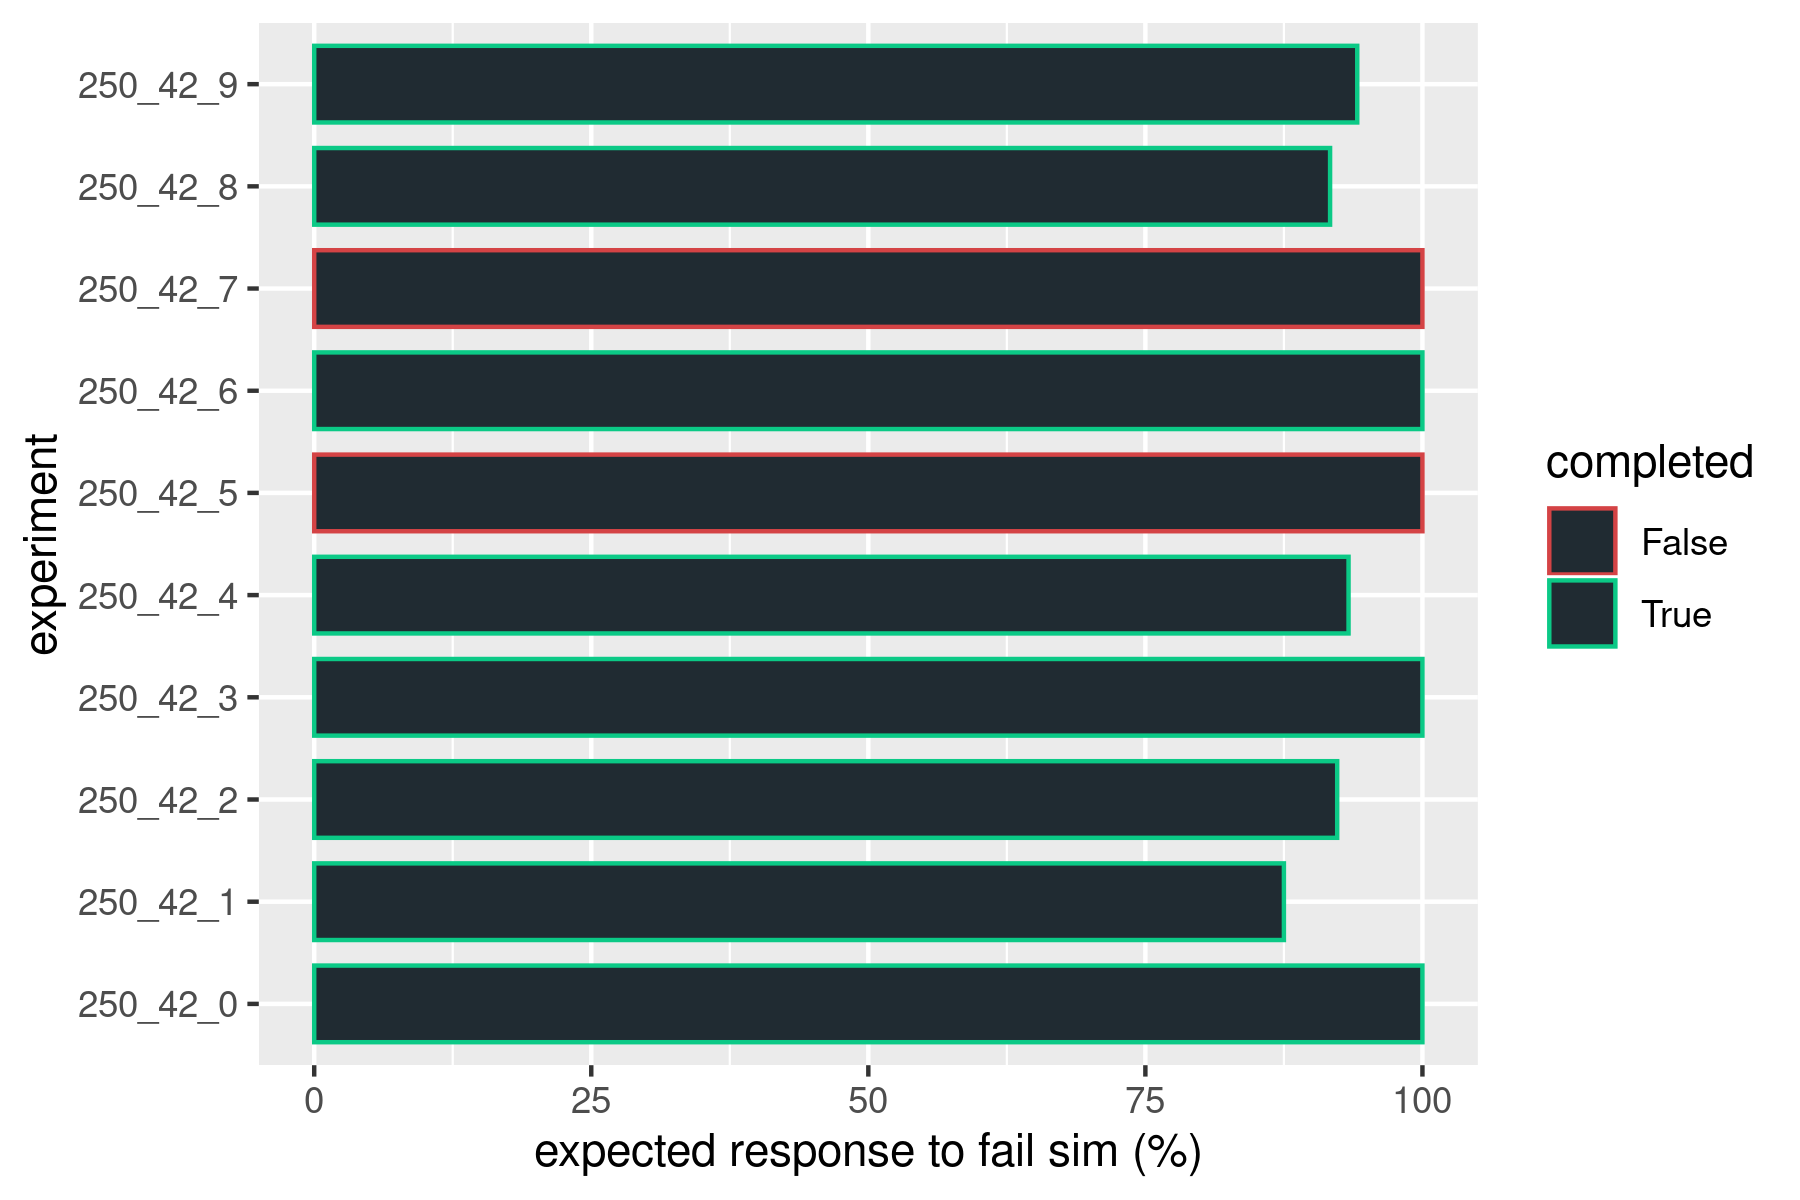
\includegraphics[width=\textwidth]{img/expected_res.png}
        \caption{\textsc{Expected Response}}
        \label{fig:expected_res}
    \end{subfigure}
    \hfill
    \begin{subfigure}[b]{0.49\textwidth}
        \centering
        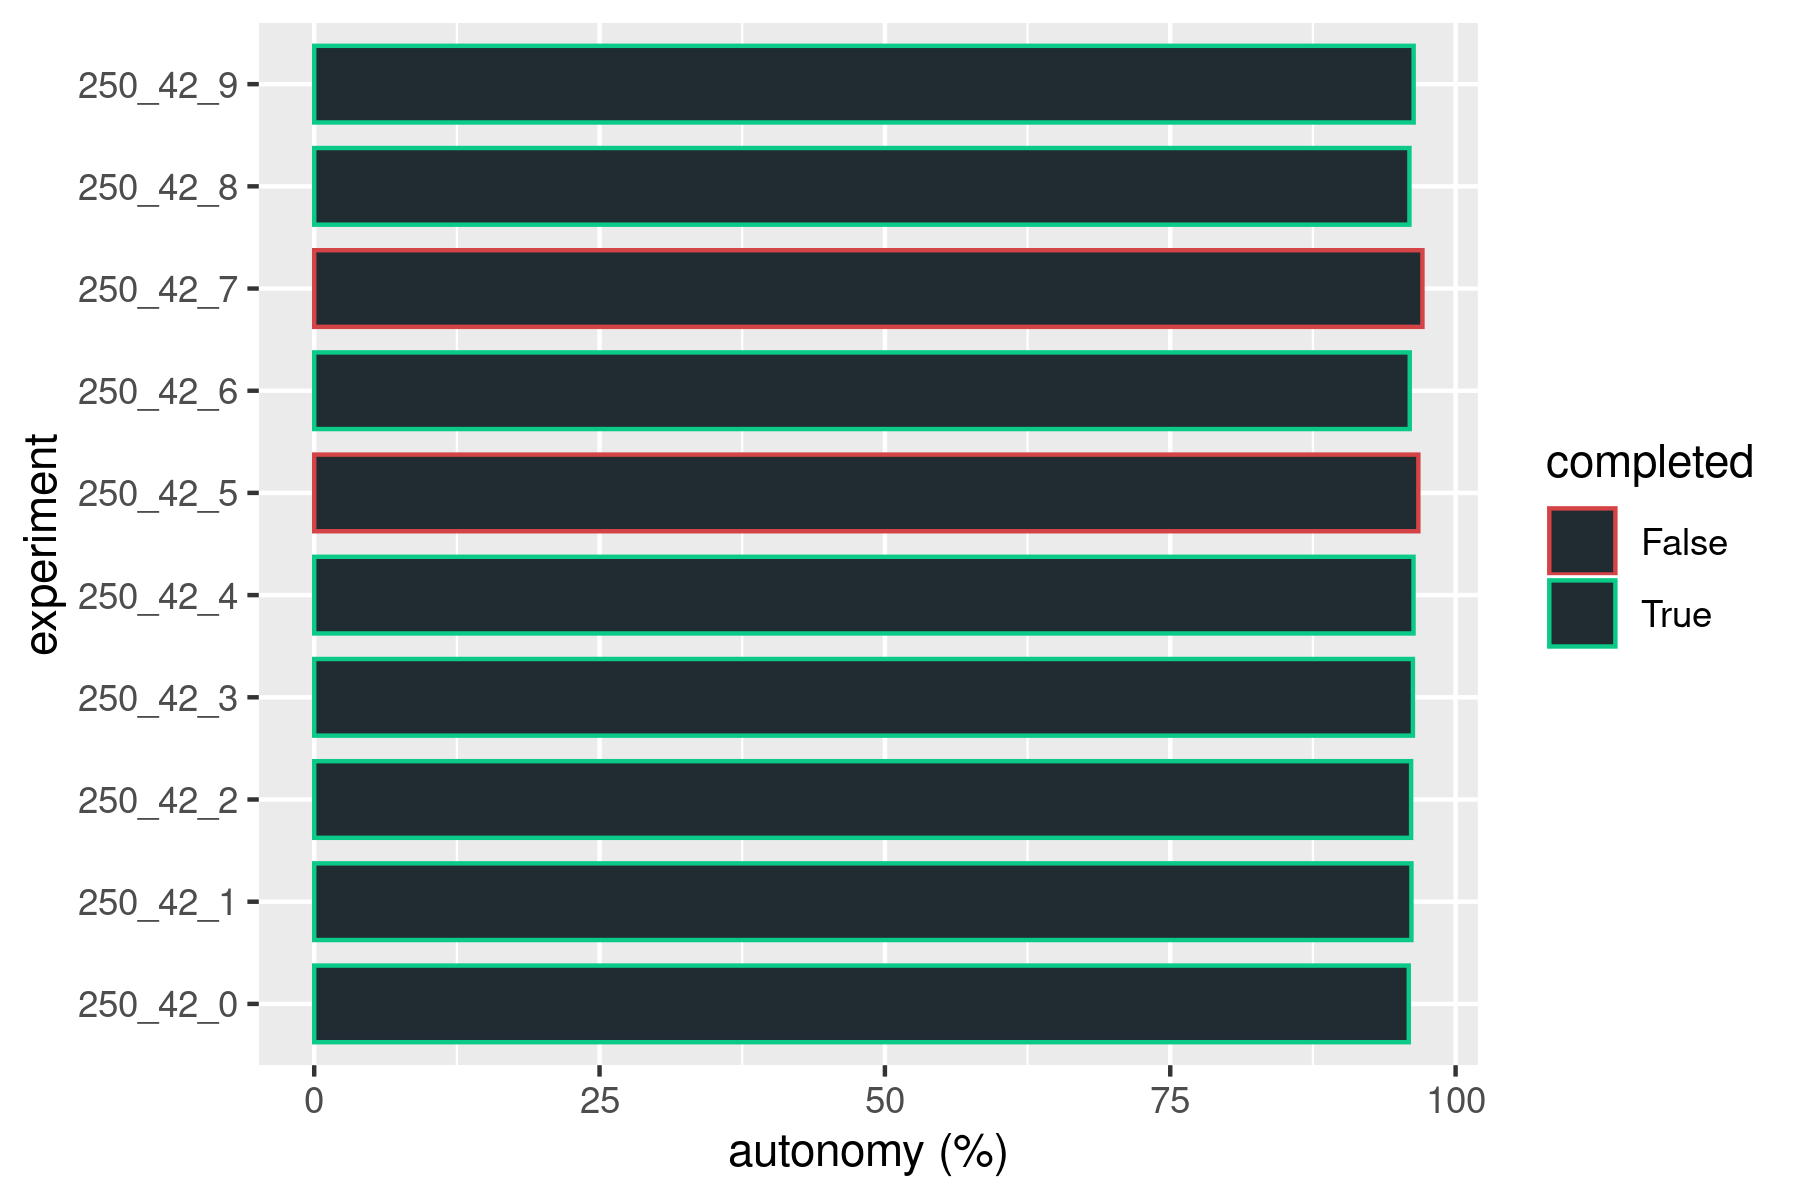
\includegraphics[width=\textwidth]{img/autonomy_percentage.png}
        \caption{\textsc{Autonomy Percentage}}
        \label{fig:autonomy_percentage}
    \end{subfigure}
\caption{\textsc{Evaluation Results}}
\label{fig:evaluation_res}
\end{figure}
\noindent
Also revealing is the activity distribution, i.e., how much of the runtime the robot spends on which activity or in which mode (cf. fig. \ref{fig:mode_times}).
This contextualizes the autonomy percentage quite well, and again it can be seen that the robot spends negligible time waiting and most of its time driving and scanning.
(Un)docking and charging naturally takes some time as well. Beyond that, some error handling (\code{cont}) can be identified.

\vfill
\pagebreak

\begin{figure}[H]
    \centering
    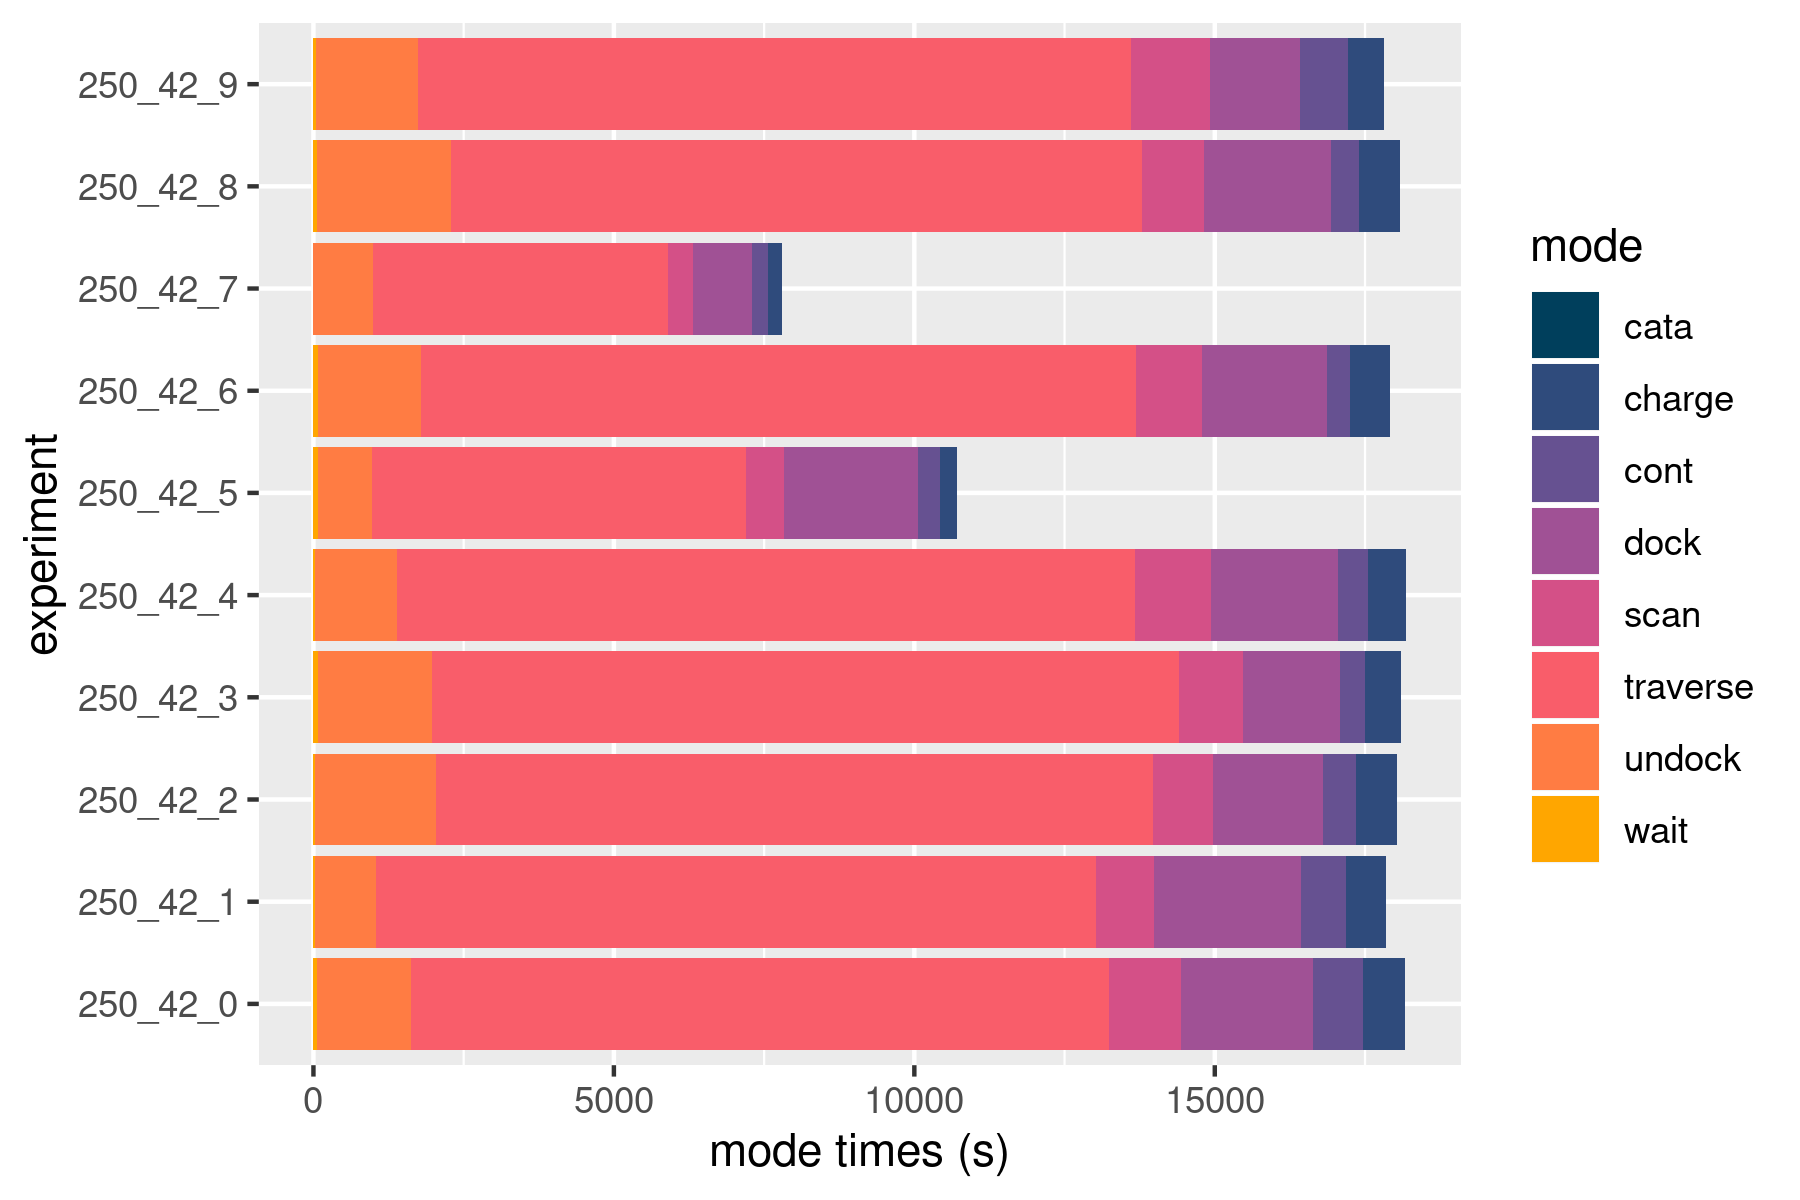
\includegraphics[width=0.65\textwidth]{img/mode_times.png}
    \caption{\textsc{Mode Distribution}}
    \label{fig:mode_times}
\end{figure}
\noindent
Based on the results, it can be concluded that the proposed framework drastically improves the resilience with respect to the identified challenges. The initial goal of assigning each
of the identified problems to a different category (cf. fig. \ref{fig:problem_types}) was achieved, and the experiments demonstrate a certain level of reliability.
The detailed results may be taken from fig. \ref{fig:detailed_monitoring_eval_res}.
